\documentclass[12pt]{article}
\usepackage[T2A]{fontenc}
\usepackage[utf8]{inputenc}
\usepackage[russian]{babel}
\usepackage[a4paper,left=2.5cm, right=1.5cm, top=2.5cm, bottom=2.5cm]{geometry}
\usepackage{graphicx}

\begin{document}
\title{Моделирование подразделений МЧС на основе
групповых объектов}

\author{Ю.В. Седельников}
\date{\today}
\maketitle

\abstract
В настоящее время для управления процессом ликвидации последствий чрезвычайных
ситуаций широко используются системы поддержки принятия решений на основе
имитационного моделирования. Такие системы представляют собой специализированные
приложения, которые позволяют работать с цифровыми картами местности путем нанесения
обстановки, проведения расчетов, манипулирования объектами.

\section{Текст}

Одной из задач при построении моделей подобных
систем является создание моделей подразделений
МЧС. Особенности функционирования таких подразделений дают возможность представить их в виде групповых объектов.
В общем случае с помощью группового объекта
можно представить имитационную модель некоторой
системы, состоящую из элементов и связей между ними, функционирующих в определенные дискреты времени. Например, на его основе можно представить пожарный расчет, войска ГО, поисково-спасательную
службу и т. д.
При построении СППР ликвидации последствий
чрезвычайных ситуаций необходимо разработать следующие модели подразделений МЧС (рис. 1).
Моделируемые подразделения МЧС имеют следующую структуру.
Поисково-спасательная служба — это подразделения, которые должны выполнять функции по проведению поисково-спасательных операций в зоне ЧС.
В СППР ее можно представить в виде информационной модели (рис. 2).
Войска ГО должны обеспечивать функции эвакуации и поддержания жизнеобеспечения населения, восстановления поврежденных объектов и коммуникаций.
Их информационная модель в СППР представлена
на рис. 3.
Пожарная охрана должна выполнять функции тушения пожаров и проведения первоочередных аварийноспасательных операций. На рис. 4 представлена ее информационная модель в СППР.
Психологическая служба должна обеспечивать
функции оказания экстренной психологической помощи пострадавшим. Ее модель представлена
на рис. 5.
«Центроспас» должен выполнять функции оперативного реагирования при возникновении ЧС, модель которых приведена на рис. 6.

\begin{figure}[h]
\center{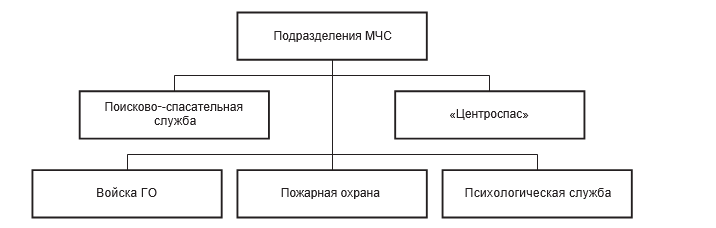
\includegraphics[scale=1]{Pics/1.png}}
\caption{Моделируемые подразделения МЧС}
\end{figure}

\begin{figure}[h]
\center{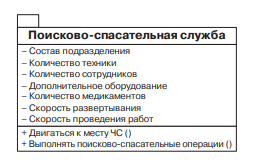
\includegraphics[scale=1]{Pics/2.png}}
\caption{Диаграмма модели поисково-спасательной
службы}
\end{figure}

\begin{figure}[h]
\center {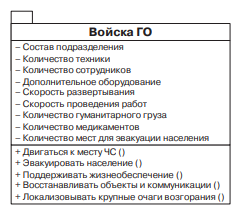
\includegraphics[scale=1]{Pics/3.png}}
\caption{Диаграмма модели войск ГО}
\end{figure}

\begin{figure}[h]
\center {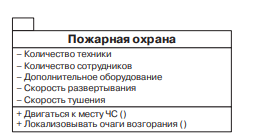
\includegraphics[scale=1]{Pics/4.png}}
\caption{Диаграмма модели пожарной охраны}
\end{figure}

\begin{figure}[h]
\center {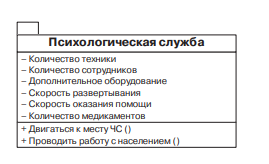
\includegraphics[scale=1]{Pics/5.png}}
\caption{Диаграмма модели психологической службы}
\end{figure}

\begin{figure}[h]
\center {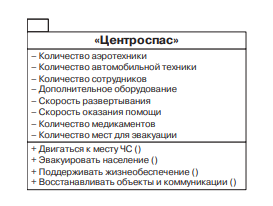
\includegraphics[scale=1]{Pics/6.png}}
\caption{Диаграмма модели «Центроспас»}
\end{figure}
\begin{itemize}
\item набирать текст;
\item управлять начертанием и размером шрифта;
\item а теперь ещё и создали список.
\end{itemize}


Необходимость описания данных моделей в виде
групповых объектов обусловлена тем, что в реальных
системах, для которых строятся указанные имитационные модели, взаимодействие осуществляется не отдельными единицами, а объединенными группами. Соответственно рассмотрение и моделирование подобных
систем должно осуществляться в контексте взаимодействия групповых объектов. В противном случае могут
быть не учтены какие-либо важные и значимые
свойства.
Моделируемые единицы представляют собой элементы подразделений, участвующих в операциях. Это
может быть колесная или гусеничная техника, летательные аппараты, стационарные единицы, расчеты
и т. д. Каждый подобный элемент имеет ряд характеристик, в частности тип элемента, назначение элемента,
функциональные возможности, технические характеристики, степень работоспособности и т. д. Элемент
группового объекта представляет собой модель физического объекта. В общем случае он может быть охарактеризован следующей совокупностью:

\[E_{i}=\langle X_{i}Y_{i}Z_{i} H_{i}G_{i} \rangle \]

 где
\[X_{i}=\{ x_{j}|j = \overline{1,NX}\}\]
 — множество входных сигналов элемента;
\[Y_{i}=\{ y_{j}|j = \overline{1,NY}\}\]
множество выходных сигналов элемента ;
\[Z_{i}=\{ z_{j}|j = \overline{1,NZ}\}\]
 — множество состояний элемента;
\[H_{i}=\{ h_{j}|j = \overline{1,NH}\}\]
 — множество параметров элемента
(в соответствии с диаграммами); 
\[G_{i}=\{ g_{j}|j = \overline{1,NG}\}\]
— множество функций элемента.
Очевидно, что построение моделей подразделений,
состоящих из подобных элементов, связано с моделированием однотипных единиц, обладающих общими
свойствами. Это дает возможность при построении моделей объединять элементы в групповые объекты, повышая эффективность создания и управления отдельными единицами.
Групповой объект может быть охарактеризован как
множество GO независимо функционирующих однородных элементов Ei
, связанных коммуникационной
функцией F:

\[
	GO = \{ E_{i}|i = \overline{1,N}\}
\]
\[
	F \subset  \Bigg( \bigcup_{i=1}^{N}Y_{i}       \Bigg)  \times \Bigg( \bigcup_{i=1}^{N}X_{i}       \Bigg), 
\]

причем

\[
	\forall y  \in  \Bigg( \bigcup_{i=1}^{N}Y_{i}       \Bigg), x \in  \Bigg( \bigcup_{i=1}^{N}X_{i} \Bigg): yFx
\]
	

\[
\int_a^b x^2 dx = \left. \frac{x^3}{3} \right|_a^b .
\]

\section{Иллюстрации}

Вставим рисунок и сошлёмся на него (рис.~\ref{lion})

\begin{figure}[h]
\center{
\includegraphics[scale=0.5]{TeX_lion.jpg}}
\caption{Талисман \TeX, созданный художником Дуэйном Бибби}
\label{lion}
\end{figure}

\end{document}